\documentclass{article}

\usepackage{datetime}
\usepackage[utf8]{inputenc}
\usepackage[margin=30mm]{geometry}
\usepackage{graphicx}
\usepackage{mathtools}
\usepackage{tikz}
\usepackage{tikz-qtree}

\setlength{\parskip}{\medskipamount}
\setlength{\parindent}{0pt}

\begin{document}
\title{T3: Time and global state\\TDT4190}
\author{Kjetil Sletten, Simen Skoglund and Christian Peter}
\date{\today}
\maketitle
\section{Time}
\subsection*{a)}
%Hvorfor kan vi trenge både fysiske og logiske klokker i distribuerte systemer? Gi to eksempler for bruk av fysiske og logiske klokker.
Hver datamaskin har en \emph{fysisk klokke}, hver klokke kalibrerer anderledes hver for seg. I et distribuert system, så vil ikke dette fungere med henhold til synkronisering. En \emph{logisk klokke} er derfor nødvendig. En logisk klokke fungerer slik at den er uavhengig av den fysiske klokken ved at den oppdaterer en \emph{program teller}. Denne telleren fungerer som en \emph{timestamp} slik at andre prosesser over det distrubuerte systemet synkroniseres mht denne telleren. Hver prosess inkrementerer telleren før hver hendelse(Dette kan være 1 eller et annet positivt nummer).

\subsection*{b)}
\emph{Happend-before} er en relasjon mellom to hendelser. Når to hendelser skjer på samme prosess, vil hendelsen skje i forhold til den ordningen som prosessen ser dem. Ved sending av en melding til en annen prosess, vil sending forekomme som første 
\begin{itemize}
	\item $a -> j$ Nei
	\item $j -> c$ Ja, fordi regelen HB3, s. 623
	\item $k -> u$ Nei
	\item $a -> e$ Ja, fordi regelen HB3, s. 623
\end{itemize}
\subsection*{c)}
Nei, når en hendelse \emph{e} på en vilkårlig prosess sender en melding til hendelse \emph{f}, så vet vi at Lamport timestamps for hendelse e er mindre enn hendelse f, altså $L(e) < L(f)$. Så hvis vi vet at $L(e) < L(f)$ så kan vi ikke si at e->f fordi vi ikke sikkert kan si om de henger sammen. Det eneste vi vet er at timestampen til e er mindre enn f. Derfor finnes vektor klokker, fordi å håndtere denne problematikken. 
\subsection*{d)}
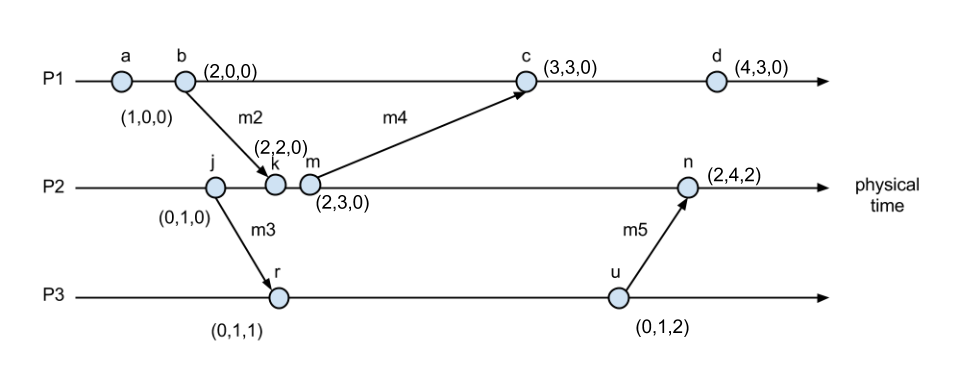
\includegraphics[scale=0.5]{Images/vector}
\subsection*{e)}
Bruker \emph{21:46:01.003} da denne har den minste RTT(28 ms). Et enkelt estimat på tiden for når prosessen skal sette klokka, tatt fra side 618: $$t + \frac{T_{round}}{2}$$ Dette gir oss en klokketid på \emph{21:46:01.017}

Siden minstetid for å sende og motta en melding vil en sette klokken til:
$$\pm (\frac{28 ms}{2} - 10 ms) = \pm 4 ms$$

Vi setter da klokken mellom \emph{21:46:01.007} og \emph{21:46:00.999}

\section{NTP Synchronization}
$T_{i-3} = 09:14:48.980$\\
$T_{i-2} = 09:14:59.030$\\
$T_{i-1} = 09:15:09.385$\\
$T_{i} = 09:15:19.425$\\

Tatt fra boken på s. 622 gir oss dette:
$$O_i = \frac{(T_{i-2} - T_{i-3} + T_{i-1} - T_i)}{2}$$
$$O_i = \frac{10050-10040}{2} = \frac{10}{2} = 5 ms$$
\section{Global State}
\begin{tikzpicture}
	\node{$S_{00}$}
	child {node (S10) {$S_{10}$}
		child {node (S20) {$S_{20}$}
			child {node (S30) {$S_{30}$}
				child {node (S31) {$S_{31}$}
					child {node (S32) {$S_{32}$}
						child {node (S33) {$S_{33}$}
							child {node (S43) {$S_{43}$}
								child {node (S44) {$S_{44}$}}}
							child {node (S34) {$S_{34}$}}}}}}
			child {node (S21) {$S_{21}$}
				child {node (S22) {$S_{22}$}
					child {node (S23) {$S_{23}$}}}}}
		child {node (S11) {$S_{11}$}}}
	child {node (S01) {$S_{01}$}
	};
	\draw (S01) -- (S11);
	\draw (S11) -- (S21);
	\draw (S21) -- (S31);
	\draw (S34) -- (S44);
	\draw (S22) -- (S32);
	\draw (S23) -- (S33);

\end{tikzpicture}
\section{Snapshot}
Det som skjer når A starter snapshot algoritmen er:
\begin{enumerate}
	\item A sender en melding med tilstand 21(for C1) til B.
	\item A lagrer tilstanden sin til 21.
	\item A sender en markørmelding til B.
	\item B mottar markørmeldingen.
	\item B finner ut at den nye tilstanden nå er 22.
	\item B lagrer tilstanden som skjer når markørmeldingen er motatt.
	\item B sender en markørmelding til A.
	\item A mottar B sin markørmelding.
	\item A lagrer C2 sin tilstand som nå er 22.
\end{enumerate}
\end{document}